\documentclass[10pt, aspectratio=169]{beamer}

\usetheme[progressbar=frametitle]{metropolis}

\usepackage[utf8]{inputenc}
\usepackage{lmodern}
\usepackage{appendixnumberbeamer}
\usepackage{xcolor}
\usepackage{subcaption}
\usepackage{tikz}
\usepackage{bm}
\usepackage{booktabs}


\usetikzlibrary{arrows,positioning}

\mode<presentation>
% enable the following row to show notes for training your talk
%\setbeameroption{show notes on second screen}


\definecolor{rwthblue}{RGB}{0,84,159}
\definecolor{rwthmagenta}{RGB}{227,0,102}
\definecolor{rwthyellow}{RGB}{255,237,0}
\definecolor{rwthgreen}{RGB}{87,171,39}
\definecolor{rwthred}{RGB}{204,7,30}

\setbeamercolor{normal text}{fg=rwthblue, bg=white}
\setbeamercolor{alerted text}{fg=rwthmagenta}
\setbeamercolor{example text}{fg=rwthyellow}

\newcommand{\source}[1]{
  \begin{tikzpicture}[remember picture, overlay]
    \node[xshift=0cm, yshift=-.3cm, above=of current page.south] {\footnotesize Source: #1};
  \end{tikzpicture}
}

\tikzset{basic/.style={draw,fill=none,
                       text badly centered,minimum width=3em}}
\tikzset{input/.style={basic,circle,minimum width=3.5em}}
\tikzset{weights/.style={basic,rectangle,minimum width=2em}}
\tikzset{functions/.style={basic,circle, minimum width=3em}}

\title{Long Short-Term Memory}
\subtitle{Joint Proseminar on Machine Learning and Image Processing}
\date{\today}
\author{Fynn Jansen, Leon Benz}
\institute{Chair of Computer Science 13 (Computer Vision)\\RWTH Aachen}
\makeatletter
\setbeamertemplate{frame footer}{Long Short-Term Memory \hfill Fynn Jansen, Leon Benz, RWTH}
\makeatother

\begin{document}

\maketitle

% ----------------------------------------------------------------

% Contents
\begin{frame}[t]{Contents}
\begin{itemize}
    \item \textbf{Introduction}
    \item Background
    \item Naive Solution
    \item LSTM Architecture
    \item Variants
    \item LSTM vs Transformer
    \item Applications
    \item Discussion
    \item Conclusion
\end{itemize}
\end{frame}

%Introduciton
\begin{frame}[t]{Introduction - The importance of Sequence Data}
Real world data often best described by sequences: \pause
\begin{itemize}
    \item Language \pause
    \item Music \& Audio \pause
    \item (Stock) prices \pause
    \item Weather \pause
\end{itemize}
Recurrent Neural Networks: Pick up on patterns in sequences\pause \\
In practice: Difficult to train 
\end{frame}

% Background
\begin{frame}[t]{Contents}
\begin{itemize}
    \item Introduction
    \item \textbf{Background}
    \item Naive Solution
    \item LSTM Architecture
    \item Variants
    \item LSTM vs Transformer
    \item Applications
    \item Discussion
    \item Conclusion
\end{itemize}
\end{frame}


\begin{frame}[t]{Background – Neural Networks}
\begin{itemize}
  \item Artificial neurons: simplified models of biological neurons
    \pause
  \item A \textbf{perceptron} computes a weighted sum of inputs:
    \[
      y = f\left(\sum_{i=0}^{n}{w_ix_i + b}\right)
    \]
    \pause
  \item Non-linearity introduced via activation function $f$
\end{itemize}
\end{frame}

\begin{frame}[t]{Background - Neural Networks}
\begin{center}
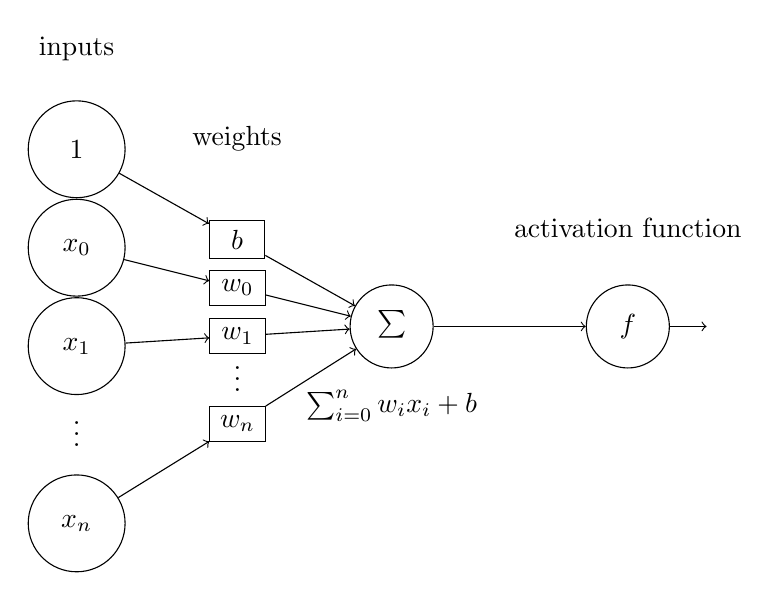
\begin{tikzpicture}
    % Draw input nodes
    \foreach \h [count=\hi ] in {$x_1$,$x_0$,$1$}{%
          \node[input] (f\hi) at (0,\hi*1.25cm-1.5 cm) {\h};
        }
    % Dot dot dot ... x_n
    \node[below=0.62cm] (idots) at (f1) {\vdots};
    \node[input, below=0.62cm] (last_input) at (idots) {$x_n$};
    % Draw summation node
    \node[functions] (sum) at (4,0) {\Huge$\sum$};
    \node[below=0.69cm] at (sum) {$\sum_{i=0}^n w_ix_i + b$};
    % Draw edges from input nodes to summation node
    \foreach \h [count=\hi ] in {$w_1$,$w_0$,$b$}{%
          \path (f\hi) -- node[weights] (w\hi) {\h} (sum);
          \draw[->] (f\hi) -- (w\hi);
          \draw[->] (w\hi) -- (sum);
        }
    % Dot dot dot ... w_n
    \node[below=0.05cm] (wdots) at (w1) {\vdots};
    \node[weights, below=0.45cm] (last_weight) at (wdots) {$w_n$};
    % Add edges for last node and last weight etc
    \path[draw,->] (last_input) -- (last_weight);
    \path[draw,->] (last_weight) -- (sum);
    % Draw node for activation function
    \node[functions] (activation) at (7,0) {$f$};

    \draw[->] (sum) -- (activation);
    \draw[->] (activation) -- ++(1,0);
    % Labels
    \node[above=1cm]  at (f3) {inputs};
    \node[above=1cm] at (w3) {weights};
    \node[above=1cm] at (activation) {activation function};
\end{tikzpicture}
\end{center}
\end{frame}

\begin{frame}[t]{Background - Neural Networks}

Perceptrons are combined into multi-layer neural networks (MLPs)
\begin{center}

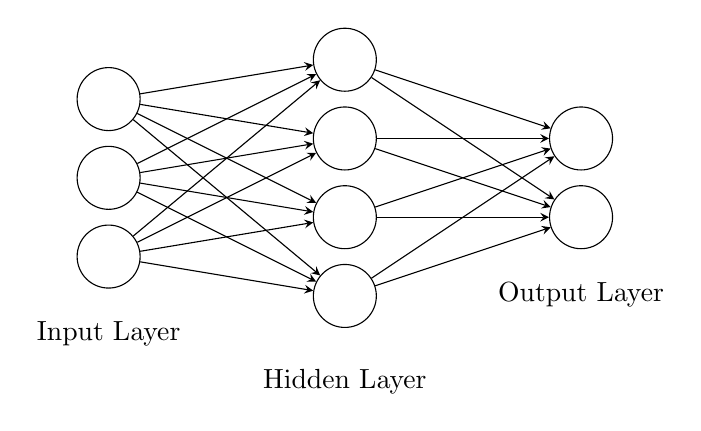
\begin{tikzpicture}[
    neuron/.style={circle, draw=black, minimum size=.8cm},
    layer/.style={minimum width=2cm, align=center},
    ->, >=stealth
  ]

  % Input Layer
  \node[neuron] (I1) at (0,1) {};
  \node[neuron] (I2) at (0,0) {};
  \node[neuron] (I3) at (0,-1) {};
  \node[below=0.3cm of I3] (ILabel) {Input Layer};

  % Hidden Layer
  \foreach \i in {1,...,4}
    \node[neuron] (H\i) at (3, 2.5-\i*1) {};

  \node[below=0.4cm of H4] (HLabel) {Hidden Layer};

  % Output Layer
  \node[neuron] (O1) at (6,0.5) {};
  \node[neuron] (O2) at (6,-0.5) {};
  \node[below=0.3cm of O2] (OLabel) {Output Layer};

  % Connections Input -> Hidden
  \foreach \i in {1,2,3}
    \foreach \j in {1,2,3,4}
      \draw[->] (I\i) -- (H\j);

  % Connections Hidden -> Output
  \foreach \i in {1,2,3,4}
    \foreach \j in {1,2}
      \draw[->] (H\i) -- (O\j);

\end{tikzpicture}
\end{center}
\end{frame}

\begin{frame}[t]{Background – Training Neural Networks}
\begin{itemize}
  \item Neural networks learn by minimizing a \textbf{loss function}
    \pause
  \item Use \textbf{stochastic gradient descent} (SGD):
    \[
      \theta \leftarrow \theta - \eta \nabla_\theta L(\theta)
    \]
    \pause
  \item Gradients are computed using \textbf{backpropagation}
    \pause
  \item Works well for fixed-size input/output — not ideal for sequences
\end{itemize}
\source{LeCun et al. 1998}
\end{frame}

\begin{frame}[t]{Background – Recurrent Neural Networks}
\begin{itemize}
  \item Designed to process sequences of arbitrary length
    \pause
  \item Maintain a \textbf{hidden state} $h_t$ to capture temporal context
    \pause
  \item Reuse weights across time steps
    \pause
  \item Core equations:
    \[
      h_t = \varphi(W_h x_t + U_h h_{t-1} + b_h)
      \qquad
      y_t = \psi(W_y h_t + b_y)
    \]
    \pause
\end{itemize}
\begin{center}
  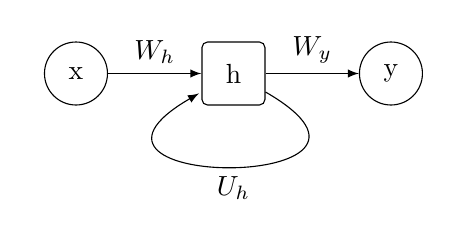
\begin{tikzpicture}[>=latex,
    % styles for clarity
    input/.style   ={draw, circle, minimum size=8mm},
    hidden/.style  ={draw, rectangle, rounded corners=2pt, minimum size=8mm},
    output/.style  ={draw, circle, minimum size=8mm},
    node distance = 2cm
  ]
    \node[input](x) at (0,0) {x};
    \node[hidden](h) at (2,0) {h};
    \node[output](o) at (4, 0) {y};

    \draw[->] (x) -- node[above]{$W_h$} (h);
    \draw[->] (h) -- node[above]{$W_y$} (o);
    \path
      (h) edge[->,
            out=-30,
            in=-150,
            looseness=7,
            loop]
            node[below]{$U_h$}
      (h);
  \end{tikzpicture}
\end{center}
\source{Elman 1990}
\end{frame}

\begin{frame}[t]{Background – Unrolling an RNN}
\begin{itemize}
  \item RNNs can be visualized as a sequence of repeated cells
    \pause
  \item Each time step processes one input and updates the hidden state
    \pause
  \item Hidden state carries memory across time
\end{itemize}
\begin{center}
  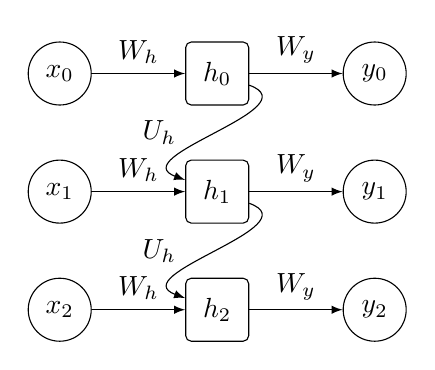
\begin{tikzpicture}[>=latex,
      % styles for clarity
      input/.style   ={draw, circle, minimum size=8mm},
      hidden/.style  ={draw, rectangle, rounded corners=2pt, minimum size=8mm},
      output/.style  ={draw, circle, minimum size=8mm},
      node distance = 2cm
    ]
    \foreach \t [count=\i from 1] in {0,1,2}{
      % place nodes at (0,-2*\i), (2,-2*\i), (4,-2*\i)
      \node[input]  (x\i) at (0,-1.5*\i) {$x_{\t}$};
      \node[hidden] (h\i) at (2,-1.5*\i) {$h_{\t}$};
      \node[output] (o\i) at (4,-1.5*\i) {$y_{\t}$};

      % input → hidden and hidden → output
      \draw[->] (x\i) -- node[above] {$W_h$} (h\i);
      \draw[->] (h\i) -- node[above] {$W_y$} (o\i);

      % hidden_{t–1} → hidden_t for t>0
      \ifnum\i>1
        \pgfmathtruncatemacro{\j}{\i-1}
        \draw[->, out=-20, in=160, looseness=1.5]
          (h\j) to node[left=.4cm] {$U_h$} (h\i);
      \fi
    }
  \end{tikzpicture}
\end{center}
\source{Elman 1990}
\end{frame}

\begin{frame}[t]{Background – Backpropagation Through Time}
\begin{itemize}
  \item To train RNNs, we apply \textbf{Backpropagation Through Time (BPTT)}
    \pause
  \item Compute gradients of loss at each time step $t$ w.r.t. previous states
    \pause
  \item The gradient of the loss at time $T$ w.r.t. a hidden state $h_t$:
    \[
    \frac{\partial \mathcal{L}_T}{\partial h_t} = \sum_{k=t}^T \left( \frac{\partial \mathcal{L}_T}{\partial h_k} \cdot \prod_{j=t+1}^{k} \frac{\partial h_j}{\partial h_{j-1}} \right)
    \]
    \pause
  \item Each $\frac{\partial h_j}{\partial h_{j-1}}$ is a Jacobian matrix
\end{itemize}
\source{Werbos 1990; Pascanu et al. 2013}
\end{frame}

\begin{frame}[t]{Background – Vanishing and Exploding Gradients}
\begin{itemize}
  \item When multiplying many Jacobians, gradients can:
  \begin{itemize}
    \item \textbf{Shrink rapidly} $\Rightarrow$ vanish
    \item \textbf{Grow uncontrollably} $\Rightarrow$ explode
  \end{itemize}
  \pause
  % \item This occurs along the \textbf{diagonal of the product of Jacobians}
  %   \begin{itemize}
  %     \item Repeated multiplication emphasizes dominant eigenvalues
  %   \end{itemize}
  % \pause
  \item In practice: RNNs \textbf{forget early inputs} and may become unstable
  \pause
  \item \textbf{Gradient clipping} can limit explosion, but not vanishing
  \pause
  \item → We need an \textbf{architectural solution}
\end{itemize}
\source{Hochreiter 1991; Pascanu et al. 2013}
\end{frame}

% Constant Error Carousel
\begin{frame}[t]{Contents}
\begin{itemize}
    \item Introduction
    \item Background
    \item \textbf{Naive Solution}
    \item LSTM Architecture
    \item Variants
    \item LSTM vs Transformer
    \item Applications
    \item Discussion
    \item Conclusion
\end{itemize}
\end{frame}

\begin{frame}[t]{Naive Solution - Constant Error Flow}
    \source{Hochreiter et al. 1997}
    Single Unit (\begin{math}j\end{math}) Constant Error Carousel (CEC):\pause
    \begin{itemize}
        \item Linear activation function : \begin{math}f(x)=x\end{math} \pause
        \item Feedback connection weight : \begin{math}w_{jj}=1\end{math} \pause
    \end{itemize}
    \begin{figure}
        \centering
        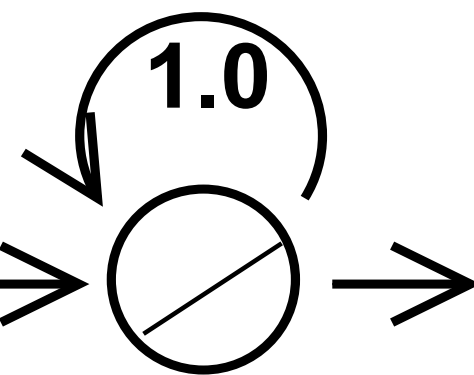
\includegraphics[width=0.25\linewidth]{images/ConstantErrorCarousel.png}
    \end{figure}
    
\end{frame}

\begin{frame}[t]{Naive Solution - Problems}
\source{Hochreiter et al. 1997}
\begin{figure}
        \centering
        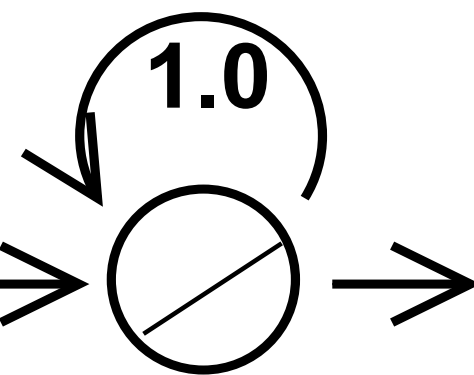
\includegraphics[width=0.25\linewidth]{images/ConstantErrorCarousel.png}
    \end{figure} \pause
Connected to other units: \pause
\begin{itemize}
    \item Input from unit $i$ \pause $\implies$ Single weight \begin{math}w_{ji}\end{math} for storing \& ignoring inputs \pause
    
    \item Output to unit $k$\pause $\implies$ Single weight \begin{math}w_{kj}\end{math} for controlling retrieval \pause
\end{itemize}
Conflicting weight update signals for \begin{math}w_{ji}\end{math} \& \begin{math}w_{kj}\end{math}\pause\begin{math}\implies\end{math} Mechanism for storage and retrieval

\end{frame}

% LSTM Architecture
\begin{frame}[t]{Contents}
\begin{itemize}
    \item Introduction
    \item Background
    \item Naive Solution
    \item \textbf{LSTM Architecture}
    \item Variants
    \item LSTM vs Transformer
    \item Applications
    \item Discussion
    \item Conclusion
\end{itemize}
\end{frame}

\begin{frame}[t]{LSTM Architecture - Gate Unit}
\source{Hochreiter et al. 1997}
Idea: Restrict flow based on context \pause
\begin{figure}
    \centering
    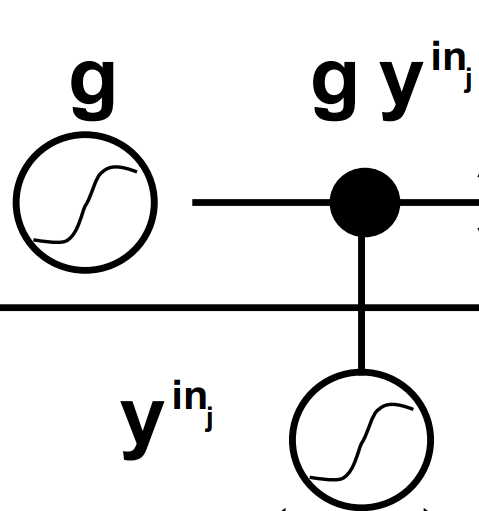
\includegraphics[width=0.2\linewidth]{images/GateUnit.png}
\end{figure} \pause
Control Input: $y^{in_j}$ \pause\\
Input gets scaled by number computed from context
\end{frame}

\begin{frame}[t]{LSTM Architecture - Memory Cell}
\source{Hochreiter et al. 1997}
Memory Cell: CEC unit with input and output gate units \pause
\begin{figure}
    \centering
    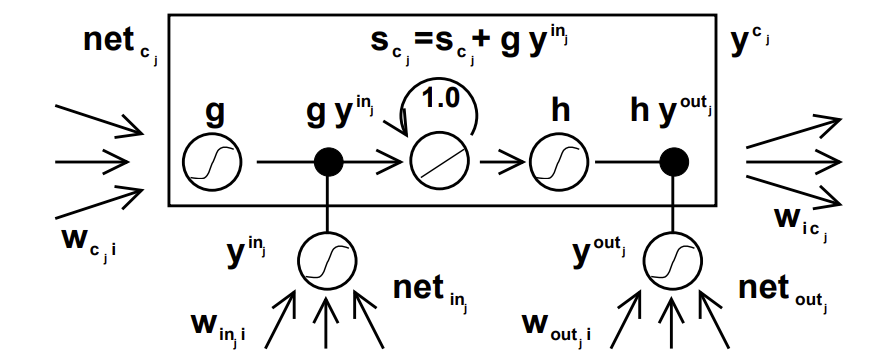
\includegraphics[width=1\linewidth]{images/LSTM-Cell-Diagram.png}
\end{figure}
\end{frame}

\begin{frame}[t]{LSTM Architecture - Network Topology}
Input for cell and gate units depend on specific implementation \pause\\
They can be:\pause
\begin{itemize}
    \item Input Units \pause
    \item Gate Units \pause
    \item Memory Cells \pause
    \item Conventional Hidden Units \pause
\end{itemize}
Commonly used topology: Inputs for Cell & Gate are all input units & memory cell outputs \pause\\
Input Gate:  \begin{math}i_t=\sigma_i\left(U_{i}h_{t-1}+W_{i} x_t + b_i\right)\end{math}\pause\\
Output Gate: \begin{math}o_t=\sigma_o\left(U_{o}h_{t-1}+W_{o}x_t + b_o\right)\end{math}\pause\\
Internal State: \begin{math}C_t=C_{t-1}+i_t\odot\sigma_c\left(U_{c}h_{t-1}+W_{x}x_t + b_c\right)\end{math}\pause\\
Output: \begin{math}h_t=o_t\odot\sigma_h\left(C_t\right)\end{math}
\end{frame}

\begin{frame}[t]{LSTM Architecture - Results}
LSTMs outperform classical RNNs in many ways:\pause
\begin{itemize}
    \item Less training examples needed\pause
    \item Higher success rate \pause
    \item Better performance on sequences that include random data \pause
    \item Better performance on noisy data \pause
    \item Can solve tasks RNNs previously could not (sequences with no local regularities)
\end{itemize}

\end{frame}

\begin{frame}[t]{LSTM Architecture - Limitations}
Drawbacks: \pause
\begin{itemize}
    \item Exploding Gradients \pause
    \item Computational Intensity \pause
    \item Limited GPU Utilization \pause
    \item Memory Bottlenecks \pause
    \item Worse performance on short sequences \pause
    \item State can not be reset
\end{itemize}
\end{frame}

% LSTM Variants
\begin{frame}[t]{Contents}
\begin{itemize}
    \item Introduction
    \item Background
    \item Naive Solution
    \item LSTM Architecture
    \item \textbf{Variants}
    \item LSTM vs Transformer
    \item Applications
    \item Discussion
    \item Conclusion
\end{itemize}
\end{frame}

\begin{frame}[t]{Variants - LSTM with forget gate}
\source{Gers et al. 1999}
Forget Gate: \pause
\begin{itemize}
    \item "Forgetting" by resetting state \pause
    \item Achieved by gating the previous state \pause
    \item \begin{math}f_t=\sigma_i\left(U_{f}h_{t-1}+W_{f} x_t + b_f\right)\end{math} \pause
    \item \begin{math}C_t=f_t\odot C_{t-1}+i_t\odot\sigma_c\left(U_{c}h_{t-1}+W_{x}x_t + b_c\right)\end{math}
\end{itemize}


\end{frame}

\begin{frame}[t]{Variants - LSTM with forget gate}
    \begin{figure}
        \centering
        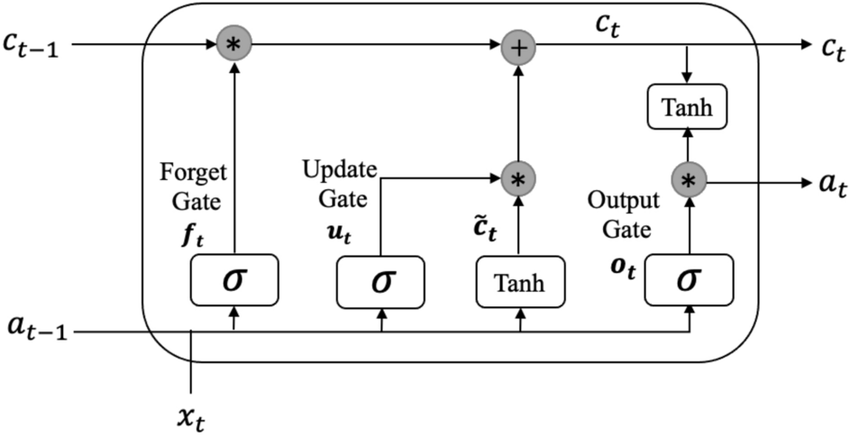
\includegraphics[\linewidth]{images/Structure-of-LSTM-cell-which-introduces-three-special-gates-Input-Gate-i-Forget-Gate.png}
    \end{figure}
\source{Nguyen et al. 2022}
\end{frame}

\begin{frame}[t]{Variants - Bidirectional LSTM}
\begin{itemize}
  \item Standard LSTM processes sequence \textbf{left to right}
    \pause
  \item Bidirectional LSTM (BiLSTM) runs \textbf{two LSTMs}:
    \begin{itemize}
      \item One forward ($\rightarrow$)
      \item One backward ($\leftarrow$)
    \end{itemize}
    \pause
  \item Output combines both:
  \[
    h_t = [\overrightarrow{h}_t; \overleftarrow{h}_t]
  \]
    \pause
\item Can use \textbf{past and future} context → better performance in many NLP tasks
\end{itemize}
\end{frame}


\begin{frame}[t]{Variants - Bidirectional LSTM}
\begin{center}
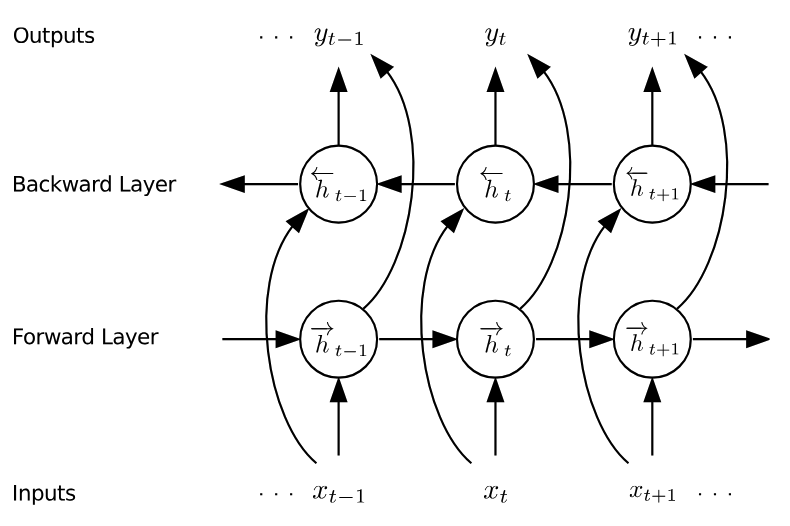
\includegraphics[width=0.7\linewidth]{images/brnn.png}
\end{center}
% \begin{itemize}
%   \item Input sequence flows through both directions
%     \pause
%   \item Outputs are concatenated or summed
%     \pause
%   \item Common in e.g. Speech, NER, Translation
% \end{itemize}
\source{Graves \& Schmidhuber 2005}
\end{frame}

\begin{frame}[t]{Gated Recurrent Unit}
\begin{itemize}
  \item GRU is a \textbf{simplified version of LSTM} with fewer gates
  \pause
  \item Uses:
    \begin{itemize}
      \item an \textbf{update gate} → controls how much past info to keep
      \item a \textbf{reset gate} → controls how much past info to forget
    \end{itemize}
  \pause
  \item Learns to balance:
    \begin{itemize}
      \item remembering important past features
      \item reacting to new input
    \end{itemize}
  \pause
  \item Often performs well with:
    \begin{itemize}
      \item less data
      \item shorter sequences
      \item faster training needs
    \end{itemize}
\end{itemize}
\source{Cho et al. 2014}
\end{frame}

\begin{frame}[t]{GRU vs. LSTM}
\begin{itemize}
  \item \textbf{LSTM}
  \begin{itemize}
    \item Uses a separate memory cell \( c_t \)
    \item Has input and output gates (forget gate was added later)
    \item Two internal states: \( h_t \) and \( c_t \)
  \end{itemize}
  \pause
  \item \textbf{GRU}
  \begin{itemize}
    \item Merges cell and hidden state into a single \( h_t \)
    \item Uses update and reset gates
    \item Simpler architecture, faster training
  \end{itemize}
\end{itemize}
\vspace{1em}
\textit{GRU simplifies LSTM by merging its memory and control into fewer components.}
\end{frame}

% LSTM vs Transformer
\begin{frame}[t]{Contents}
\begin{itemize}
    \item Introduction
    \item Background
    \item Naive Solution
    \item LSTM Architecture
    \item Variants
    \item \textbf{LSTM vs Transformer}
    \item Applications
    \item Discussion
    \item Conclusion
\end{itemize}
\end{frame}

\begin{frame}[t]{LSTM vs. Transformer – Motivation}
\begin{itemize}
  \item LSTMs have been widely used for sequence modeling since the 1990s
    \pause
  \item In recent years, \textbf{Transformers} have become the dominant model in NLP and beyond
    \pause
  \item Transformers offer a different approach: no recurrence, full attention
\end{itemize}
\source{Vaswani et al. 2017}
\end{frame}

\begin{frame}[t]{Transformers – Self-Attention Mechanism}
\begin{itemize}
  \item Core idea: Each word \textbf{attends to all others} in the input
    \pause
  \item Use \textbf{self-attention} to compute weighted combinations of all inputs
    \pause
  \item Attention weights learned dynamically — no recurrence
    \pause
  \item Enables \textbf{parallelization} and efficient learning of long-range dependencies
\end{itemize}
\pause
\begin{center}
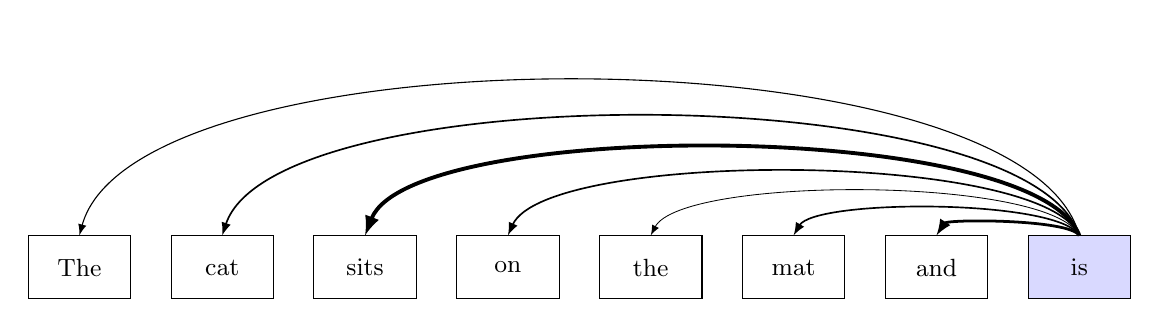
\begin{tikzpicture}[node distance=0.8cm and 0.5cm, every node/.style={font=\small}, >=latex]

  % Tokens
  \node (t1) [draw, minimum height=0.8cm, minimum width=1.3cm] {The};
  \node (t2) [draw, right=of t1, minimum height=0.8cm, minimum width=1.3cm] {cat};
  \node (t3) [draw, right=of t2, minimum height=0.8cm, minimum width=1.3cm] {sits};
  \node (t4) [draw, right=of t3, minimum height=0.8cm, minimum width=1.3cm] {on};
  \node (t5) [draw, right=of t4, minimum height=0.8cm, minimum width=1.3cm] {the};
  \node (t6) [draw, right=of t5, minimum height=0.8cm, minimum width=1.3cm] {mat};
  \node (t7) [draw, right=of t6, minimum height=0.8cm, minimum width=1.3cm] {and};
  \node (t8) [draw, fill=blue!15, right=of t7, minimum height=0.8cm, minimum width=1.3cm] {is};

  % Attention arcs (thickness represents attention weight)
  \draw[->, line width=0.4pt] (t8.north) to[out=105, in=75, looseness=0.55] (t1.north);
  \draw[->, line width=0.6pt] (t8.north) to[out=108, in=72, looseness=0.5] (t2.north);
  \draw[->, line width=1.4pt] (t8.north) to[out=111, in=69, looseness=0.45] (t3.north); % highest attention
  \draw[->, line width=0.6pt] (t8.north) to[out=114, in=66, looseness=0.42] (t4.north);
  \draw[->, line width=0.3pt] (t8.north) to[out=117, in=63, looseness=0.40] (t5.north); % lowest attention
  \draw[->, line width=0.6pt] (t8.north) to[out=120, in=60, looseness=0.38] (t6.north);
  \draw[->, line width=1.0pt] (t8.north) to[out=123, in=57, looseness=0.35] (t7.north);

\end{tikzpicture}
\end{center}
\source{Vaswani et al. 2017}
\end{frame}

\begin{frame}[t]{LSTM vs. Transformer – Comparison}
\vspace{1em}
\begin{columns}
\column{0.45\textwidth}
\textbf{LSTM}
\begin{itemize}
  \item Recurrence-based
  \item Hidden state carries memory
  \item Sequential processing
  \item Better on smaller data
  \item Fewer resources needed
\end{itemize}

\column{0.45\textwidth}
\textbf{Transformer}
\begin{itemize}
  \item Attention-based
  \item Global context at each step
  \item Fully parallelizable
  \item Excels with large datasets
  \item High compute demand
\end{itemize}
\end{columns}
\end{frame}

%LSTM Applications
\begin{frame}[t]{Contents}
\begin{itemize}
    \item Introduction
    \item Background
    \item Naive Solution
    \item LSTM Architecture
    \item Variants
    \item LSTM vs Transformer
    \item \textbf{Applications}
    \item Discussion
    \item Conclusion
\end{itemize}
\end{frame}

\begin{frame}[t]{Application – Speech Recognition}
\begin{itemize}
  \item Spoken language is a sequence of sounds that unfolds over time
  \pause
  \item LSTMs can learn how current sounds depend on earlier ones:
    \begin{itemize}
      \item e.g. understanding that "s" at the end of “cats” depends on earlier phonemes
    \end{itemize}
  \pause
  \item Bidirectional LSTMs are especially useful:
    \begin{itemize}
      \item They consider both past and future context in a sentence
      \item This helps distinguish similar sounds in different contexts
    \end{itemize}
  \pause
  \item LSTMs reduce the need for manual feature extraction
\end{itemize}
\end{frame}

%Time Series Forecasting
\begin{frame}[t]{Applications - Time Series Forecasting}
LSTMs perform better on: \pause
\begin{itemize}
    \item Long sequences \pause
    \item Complex sequences \pause
\end{itemize}
Examples: \pause
\begin{itemize}
    \item 2022: Deep LSTM Network forecasts electricity demand (1.5\% accuracy) \pause
    \item 2024: LSTM Architecture forcasts electricity prices
\end{itemize}
\end{frame}

%Music Generation

\begin{frame}[t]{Applications - Music Generation}
Music has temporal structure: \pause
\begin{itemize}
    \item Rhythms \pause
    \item Chord progressions \pause
    \item Melodic motives \pause
\end{itemize}
Easily representable as numbers\pause \\
\vspace{1em}
2002: LSTM Architecture used to compose music
\end{frame}

%Discussion
\begin{frame}[t]{Contents}
\begin{itemize}
    \item Introduction
    \item Background
    \item Naive Solution
    \item LSTM Architecture
    \item Variants
    \item LSTM vs Transformer
    \item Applications
    \item \textbf{Discussion}
    \item Conclusion
\end{itemize}
\end{frame}

\begin{frame}[t]{Discussion - the Future of LSTMs}
\source{Zhao et al. 2025}
Future of the LSTM architecture: \pause
\begin{itemize}
    \item Largely replaced by transformers in NLP and vision, but: \pause
    \begin{itemize}
        \item LSTMs still useful for small datasets (better performance) \pause
        \item LSTMs require fewer Resources \pause
        \item LSTM - Transformer hybrid architectures \pause
    \end{itemize} 
    \item Inspired many Variants and Architecture
\end{itemize}

\end{frame}

%Conclusion
\begin{frame}[t]{Contents}
\begin{itemize}
    \item Introduction
    \item Background
    \item Naive Solution
    \item LSTM Architecture
    \item Variants
    \item LSTM vs Transformer
    \item Applications
    \item Discussion
    \item \textbf{Conclusion}
\end{itemize}
\end{frame}

\begin{frame}[t]{Conclusion}
LSTM Architecture: \pause
\begin{itemize}
    \item Internal CEC unit \begin{math}\implies \end{math} Internal State (Memory) \pause
    \item Input Gate \begin{math}\implies\end{math} Protects memory from unwanted perturbation \pause
    \item Output Gate \begin{math}\implies\end{math} Controls output of the memory to other units \pause
    \item Eliminates vanishing Gradient Problem \pause
    \item Inspired many Variants and RNN Architectures \pause
\end{itemize}
Currently: \pause
\begin{itemize}
    \item Replaced by transformers in many Applications \pause
    \item Development of new LSTM based architectures \pause
    \item Remain useful in some cases 
\end{itemize}
\end{frame}

% ----------------------------------------------------------------
\nocite{alselwi2024lstmfuture}
\nocite{bolboaca2023lstmperformance}
\nocite{eck2002musicgeneration}
\nocite{gers1999forgetgate}
\nocite{gers2001timeseries}
\nocite{gokmen2018hadamard}
\nocite{gradient-clipping}
\nocite{harris1954languagestructure}
\nocite{hochreiter1997lstm}
\nocite{nielsen2024electricitypriceforcasting}
\nocite{torres2022elctricityforecasting}
\nocite{zhao2025lstmtransformerhybrid}
\nocite{zheng2018scalability}
\nocite{zheng2020scalability}
\nocite{hochreiter1991}
\nocite{elman90}
\nocite{werb1990bptt}
\nocite{pascanu2013rnntraining}
\nocite{vaswani2017attention}

\setbeamerfont{bibliography item}{size=\footnotesize}
\setbeamerfont{bibliography entry author}{size=\footnotesize}
\setbeamerfont{bibliography entry title}{size=\footnotesize}
\setbeamerfont{bibliography entry location}{size=\footnotesize}
\setbeamerfont{bibliography entry note}{size=\footnotesize}
\begin{frame}[allowframebreaks]{References}

  \bibliographystyle{alpha}
  \bibliography{slides}

\end{frame}
\end{document}
